%\documentclass[12pt]{report}
%\documentclass[12pt]{extreport}
\documentclass[17pt]{extarticle}
\usepackage{graphicx}
\usepackage{setspace}
\usepackage{amsmath,amssymb}
\usepackage{IEEEtrantools}
\usepackage{cancel}

\usepackage{geometry}
 \geometry{
 a4paper,
 total={170mm,264mm},
 left=20mm,
 top=10mm,
 }

\begin{document}


\section{Relativit\'a galileiana}










Uno stesso corpo pu\'o essere contemporaneamente in moto o fermo se a osservarlo sono due soggetti diversi, per questo \'e necessario specificare il sistema di riferimento scelto. \emph{Le Trasformazioni Galileiane si occupano di ricavare le relazioni matematiche sussistenti di una stessa grandezza osservata da due sistemi di riferimento differenti}. 

Il pi\'u semplice esempio di sistema ove applicare una trasformazione galileiana \'e dato da un corpo, ad esempio un orso polare, che si muove su un sistema di riferimento (ad esempio la lastra di ghiaccio ove cammina), che a sua volta \'e in moto rettilineo uniforme rispetto ad un altro sistema di riferimento, ad esempio un sistema di riferimento \emph{solidale} con la terra ferma.

Stando sulla terra ferma, del moto di questo orso distinguiamo
\begin{enumerate}
	\item spostamento relativo $\Delta\vec{S}_r$, ossia lo spostamento dell'orso rispetto alla lastra;
	\item spostamento di trascinamento $\Delta\vec{S}_t$, ossia lo spostamento della lastra rispetto alla terra ferma.
\end{enumerate}

Ciascuno spostamento avverr\'a ad una differente velocit\'a che chiamiamo, rispettivamente, velocit\'a relativa $\vec{v}_r$ e velocit\'a di trascinamento $\vec{v}_t$.


In questo esempio la trasformazione galileiana consiste nella seguente formula:

\begin{eqnarray}\label{eq:galileo}
	\vec{v}_{tf} = \vec{v}_r + \vec{v}_t
\end{eqnarray}

{\bf La velocit\'a dell'orso rispetto alla terra ferma $\vec{v}_{tf}$ \'e la somma della velocit\'a relativa e della velocit\'a di trascinamento.} \'E bene osservare che tale somma \'e vettoriale e, in generale, per essere effettuata, necessita l'uso della regola del parallelogramma.

Le trasformazioni galileiane sembrerebbero molto semplici, in realt\'a questo genere di analisi, si pu\'o complicare enormemente quando si presentano sistemi di riferimento che sono in moto l'uno rispetto all'altro 

\begin{itemize}
	\item con moti che si svolgono in tre dimensioni anzich\'e uno soltanto;
	\item moti che \emph{non} sono semplicemente rettilinei uniformi;
	\item sistemi di riferimento che \emph{non} sono necessariamente concordi ma, anzi, possono essere ruotati l'uno rispetto all'altro di un angolo $\alpha$ (fig \ref{fig:sample_figure});
	\item sistemi di riferimento che possono anche ruotare l'uno rispetto all'altro (pensare al sistema di riferimento solidale alla terra con quello solidale al sole).
\end{itemize}






\begin{tabular}{p{\textwidth}}		
	\centering
   	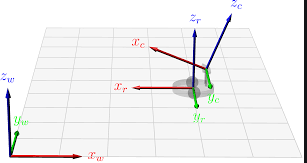
\includegraphics[width=2.5in]{SistRifDiscordi.png}
   	\label{fig:sample_figure}		
\end{tabular}



Inoltre, per quanto i concetti della relativit\'a galileiana possano risultare ovvi, in realt\'a essi sono validi soltanto quando tutte le velocit\'a in gioco, siano esse di trascinamento o relative, sono \emph{minori di ordini di grandezza} rispetto alla velocit\'a della luce $c$.

\begin{eqnarray}
	c = 3\cdot 10^8m/s
\end{eqnarray}

\'E da notare che tale condizione \'e soddisfatta nella stragrande maggioranza delle situazioni ordinarie. Ad esempio, la velocit\'a di punta di un bolide di formula 1 \'e prossima ai $v = 400km/h$ che, convertita, diventa $v\approx 10^2m/s$, ben 1 milione di volte inferiore rispetto al valore di c!

Tale condizione viene sinteticamente espressa con la seguente relazione matematica $v<<c$. Quando, invece, questa condizione cade, allora le trasformazioni galileiane non sono pi\'u valide. In particolare, per quanto detto finora, non \'e pi\'u valida nemmeno l'equazione  \ref{eq:galileo}. In tali casi occorre sostituire la Relativit\'a di Galileo con la Relativit\'a Ristretta di Einstain\footnote{In realt\'a le teorie di relativit\'a di Einstain sono due, una concepita nel 1905 e noto come relativit\'a ristretta, che generalizza la Relativi\'a di Galileo, e una pi\'u generale concepito circa 20 anni dopo, nota  come Relativit\'a Generale di Einstain, che generalizza anche la Relativit\'a Ristretta e nel quale la forza di gravit\'a viene interpretata come dovuta alla curvatura dello spazio-tempo quando sono presenti corpi dotati di una certa massa $M$.} (1905). Tale teoria trova applicazioni non nella vita ordinaria, ma, tipicamente, in fenomeni atomici e nucleari: la velocit\'a dell'elettrone intorno al nucleo dell'atomi di idrogeno, ad esempio \'e $v_e = 2.2\cdot 10^6 m/s$, poco meno di un centesimo della velocit\'a della luce. In queste condizioni, gli effetti della relativit\'a di Einstain, seppur non dominanti, sono comunque significativi (tema noto come ''struttura fine dell'atomo di idrogeno''). La relativit\'a di Einstain entra in gioco in una grande variet\'a di altri fenomeni come, ad esempio, la risonanza magnetica nucleare e fenomeni di astrofisica quali il moto di stelle e galassie nell'universo.


\section{Sistemi di riferimento inerziali}
	
Tornando alla relativit\'a galileiana, due sistemi di riferimento sono inerziali tra di loro quando si muovono di moto rettilineo l'uno rispetto all'altro. Se ci\'o accade, allora rimane valido il \emph{Primo Principio della Dinamica} in entrambe i due sistemi di riferimento, ossia in entrambe i due casi si ha che un corpo, se non sottoposto a forze, mantiene il suo moto rettilineo uniforme. Inoltre, dal momento che rimangono invariate massa, forza e accelerazione, si deduce che anche gli altri due principi della dinamica rimangono invariati.

L'invarianza dei tre principi della dinamica costituisce il {\bf Principio di Relativit\'a di Galileo}  (pag 98): I fenomeni meccanici si svolgono nello stesso modo, cio\'e seguono le stesse leggi, in tutti i sistemi di riferimento inerziali\footnote{Studieremo pi\'u in l\'a che ci\'o non \'e valido, invece, nell'elettromagnetismo ma, anzi, risulta che la velocit\'a della luce $c$ sia una costante quando si passa da un sistema di riferimento all'altro. \'E stata questa una delle osservazioni fondamentali che ha portato Einstain a formulare la sua Teoria della Relativit\'a Ristretta.}.

\section{Relativit\'a del concetto di sistema di riferimento inerziale}

Siamo indotti a pensare che esista un sistema di riferimento privilegiato.
Infatti, potremmo pensare che un tale sistema di riferimento possa essere uno solidale con la terra. Ma la terra non si muove di moto rettilineo uniforme intorno al sole, ma anzi compie un moto che, a sua volta, \'e la composizione di due moti pressoch\'e circolari uniformi (moto intorno al sole e moto intorno a se stessa). Quindi, non potremo considerare il moto della terra come esattamente inerziale\footnote{L'accelerazione di Coriolis, responsabile, tra le altre cose, del moto a vortice dell'acqua nel rubinetto, \'e un esempio che dimostra che un sistema di riferimento solidale con la terra non \'e perfettamente inerziale.}. 
Cos\'i potremmo pensare che un sistema di riferimento perfettamente inerziale possa essere uno solidale con il sole. Ma anche il sole si muove di un moto accelerato e, per la precisione, orbita intorno a un buco nero presente al centro della nostra galassia. Quindi, in linea di principio, neanche un sistema di riferimento solidale con il sole pu\'o essere considerato un sistema di riferimento perfettamente inerziale ma, anzi, pu\'o generare delle forze apparenti. Questo genere di ragionamento lo potremmo continuare all'infinito. 




Si deduce, quindi, che \emph{non esiste un sistema di riferimento privilegiato}, ma soltanto sistemi di riferimento relativi l'uno all'altro. Inoltre, un sistema di riferimento non sar\'a mai assolutamente inerziale, ma la sua inerzialit\'a sar\'a soltanto una approssimazione di volta in volta applicabile o meno a seconda della precisione con cui vengono rilevate le grandezze fisiche in gioco e, in particolare, le forze.

Come esempio di ci\'o, abbiamo detto precedentemente che nel moto di un corpo come, ad esempio, un ciclista, l'orso di cui all'esempio iniziale, una vettura su strata o altri fenomeni di vita quotidiana, la terra \'e considerabile come un sistema di riferimento inerziale. Ma tale assunzione \'e soltanto una prima approssimazione poich\'e la terra gira intorno a se stessa (oltre che intorno al sole) e ci\'o basta per dedurre che essa non sia un sistema di riferimento assolutamente inerziale. La forza apparente pi\'u evidente che si presenta in un caso come questo \'e la forza centrifuga, la quale, alle nostre latitudini, tende a opporsi a quella gravitazionale. Tuttavia questa non \'e l'unica forza apparente e ne, tantomeno, quella pi\'u evidente. Esiste un altra forza apparente, dovuta alla rotazione della terra che prende il nome di \emph{accelerazione di Coriolis} (vedere La Fisica di Feynman per approfondimenti) ed \'e espressa dalla equazione
\begin{eqnarray}
	v_c =2\vec{\omega} \times \vec{v}
\end{eqnarray}

ossia il prodotto vettoriale del vettore velocit\'a angolare $\vec{\omega}$ \footnote{Si ricorda che, dato un moto circolare uniforme, si definisce vettore velocit\'a angolare quel vettore di lunghezza $\omega = \frac{2\pi}{T}$, perpendicolare al piano ove si svolge il moto e orientato in modo tale da ''vedere'' la rotazione svolgersi in senso antiorario.} della terra e la velocit\'a tangenziale $\vec{v}$ del corpo in un sistema di riferimento solidale con la terra stessa. Uno degli effetti pi\'u evidenti dell'accelerazione di Coriolis \'e il moto rotatorio dell'acqua nel lavandino quando si apre il rubinetto e la si fa scendere nel sifone. Pi\'u in generale, sempre a causa della forza di coriolis, un qualsiasi corpo in caduta libera \emph{non} cade necessariamente in maniera verticale verso il centro della terra, ma viene leggermente deviato trasversalmente e questa deviazione \'e tanto pi\'u accentuata quanto pi\'u ci si discosta dai poli della terra (ove a velocit\'a angolare $\omega$ e la velocit\'a di caduta sono due vettori paralleli $v$). 

\end{document}